
\section{Notifications}

While non-secure dynamic updates have been a well-known misconfiguration issue for years, DNS operators still lack of the proper incentives to act.
To incentive the action of the operators of these vulnerable resources, we conducted a series of notification experiments.

Previous studies have demonstrated that directly notifying  operators does not lead to significant remediation rates~\cite{cetin2017make}. Instead, to increase the remediation rates, we notified the national CERTs and CSIRTs responsible for the hygiene of the networks where the vulnerable DNS servers are located.
Given the high concentration of vulnerable resources in a single country, before sending out the notifications at scale, we contacted directly the Japanese CERT with whom we shared all the information related to these vulnerable resources. After contacting this CERT, we measure a considerable drop (92\%) of vulnerable domains in this country by fixing 29 of the vulnerable servers.


However, even after Japan remediated most of the domains at risk in that country, more than 5,100 servers were still vulnerable leaving more than 43,000 domains at risk being exploited.
In total we conducted 8 email notification campaigns divided into 2 different phases: \textit{Phase1} targeting CERTs and CSIRTs members of the so-called 'Trusted Introducer' community; and  \textit{Phase2} targeting national and governmental CERTs. Table~\ref{tab:notif_campaign} shows an overview of the notifications that were sent out during each phase. In total, more than 200 CERTs and CSIRTs were notified via email during the time span of 6 months. The interaction with these actors was relatively low and less than 10\% actually required additional information about the scanning process. Similarly, less than 5\% of them open an automated ticket and only in 4 occasions we were notified back when the ticket was closed.

\begin{table}[!htbp]
\centering
\caption{Summary of the notification campaigns}
\label{tab:notif_campaign}
\scalebox{.8}{
\begin{tabular}{@{}llrrr@{}}
\toprule
 & \multicolumn{1}{c}{\textbf{\begin{tabular}[c]{@{}c@{}}Notification\\ Date\end{tabular}}} & \multicolumn{1}{c}{\textbf{\begin{tabular}[c]{@{}c@{}}\#Notified\\ Entities\end{tabular}}} & \multicolumn{1}{c}{\textbf{\begin{tabular}[c]{@{}c@{}}\#Unreachable\\ Entities\end{tabular}}} & \multicolumn{1}{c}{\textbf{\#Replies}} \\ \midrule
Pilot
 & 2017-05-01 & 1 & - & \begin{tabular}[c]{@{}r@{}} 1 manual \end{tabular}\\ \midrule
\multirow{3}{*}{Phase 1} & 2017-09-06 & 44 & 2 & \begin{tabular}[c]{@{}r@{}}7 automatic\\ 16 manual\end{tabular} \\
\multicolumn{1}{c}{} & 2017-09-28 & 35 & 2 & \begin{tabular}[c]{@{}r@{}}6 automatic\\ 13 manual\end{tabular} \\
\multicolumn{1}{c}{} & 2017-10-19 & 27 & 2 & \begin{tabular}[c]{@{}r@{}}4 automatic\\ 7 manual\end{tabular} \\ \midrule
\multirow{4}{*}{Phase 2} 
 & 2018-02-14 & 168 & 5 & \begin{tabular}[c]{@{}r@{}}14 automatic \\ 40 manual \end{tabular}\\
 & 2018-02-28 & 167 & 5 &  \begin{tabular}[c]{@{}r@{}}12 automatic \\ 24 manual \end{tabular} \\
 & 2018-03-16 & 162 & 5 & \begin{tabular}[c]{@{}r@{}}12 automatic \\ 24 manual \end{tabular}  \\
 & 2018-04-12 & 76 & 5 &  \begin{tabular}[c]{@{}r@{}}7 automatic \\ 7 manual \end{tabular} \\ \bottomrule
\end{tabular}}
\end{table}

A generic overview of the impact of the notifications can be seen in Fig.~\ref{fig:ts_notif} were the number of vulnerable servers and domains at risk over time is shown.
All in all, the notifications led to a 38.99\% and 39.42\%
remediation rate of the vulnerable servers and vulnerable domains respectively. These remediation rates are significantly higher than the ones reported by previous studies and signals the need to involve CERTs and CSIRTs in the remediation of vulnerabilities.  

\begin{figure}[!hbt]
    \centering
    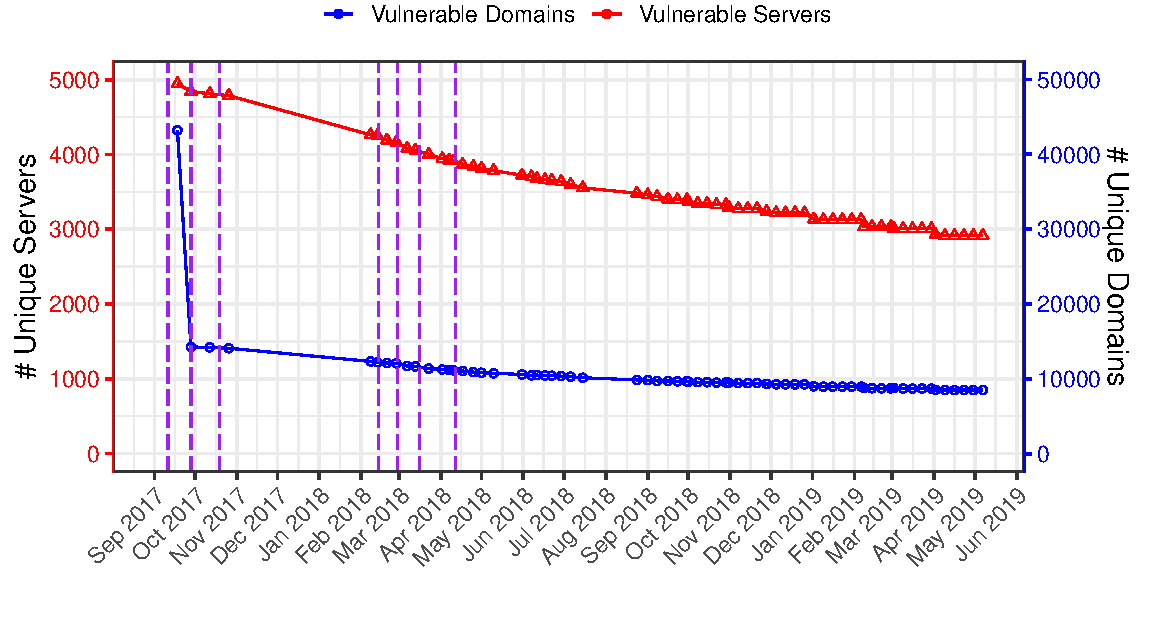
\includegraphics[width=\columnwidth]{figs/ts_notif.pdf}
    \caption{Number of vulnerable resources over time. Each dashed line represents a notification campaign.}
    \label{fig:ts_notif}
\end{figure}

\subsection{Notification methodology}



\subsection{Phase1: TF-CSIRTs}

\begin{table}[!htbp]
    \centering
    \caption{Summary statistics by the end of the Phase 1}
    \label{tab:my_label}
    \resizebox{\columnwidth}{!}{%
\begin{tabular}{lrr}
\toprule
 & TF-CSIRTs (N = 44) & Other CSIRTs (N = 36)\\
\midrule
\bf{Remediated Servers} & ~ & ~\\
\hline
~~ N (\%) & 328 (20.4)\% & 658 (19.17)\%\\
~~ max & 62 & 220\\
~~ median & 3.0 & 2.5\\
~~ mean (sd) & 7.45 $\pm$ 11.71 & 18.28 $\pm$ 39.10\\
\hline
\bf{Vulnerable Servers} & ~ & ~\\
\hline
~~ N (\%) & 1280 (79.6)\% & 2775 (80.83)\%\\
~~ max & 235 & 911\\
~~ median & 14.5 & 13.0\\
~~ mean (sd) & 29.09 $\pm$ 43.03 & 77.08 $\pm$ 172.45\\
\hline
\bf{Remediated Domains} & ~ & ~\\
\hline
~~ N (\%) & 737 (14.24)\% & 2173 (22.29)\%\\
~~ max & 108 & 847\\
~~ median & 4.0 & 4.5\\
~~ mean (sd) & 16.75 $\pm$ 27.41 & 60.36 $\pm$ 151.84\\
\hline
\bf{Vulnerable Domains} & ~ & ~\\
\hline
~~ N (\%) & 4439 (85.76\%) & 7574 (77.71\%)\\
~~ max & 1231 & 2384\\
~~ median & 29.5 & 34.0\\
~~ mean (sd) & 100.89 $\pm$ 195.19 & 210.39 $\pm$ 494.86\\
\bottomrule
\end{tabular}}
\end{table}


\begin{figure}[!hbt]
\centering
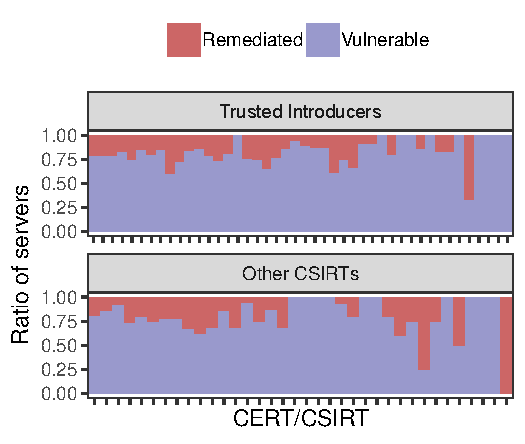
\includegraphics[width=.8\columnwidth]{distr_cleanup_1stcampaign.pdf}
\caption{Remediation rate of the DNS servers during the first campaign}
\end{figure}

\begin{figure}[!hbt]
\centering
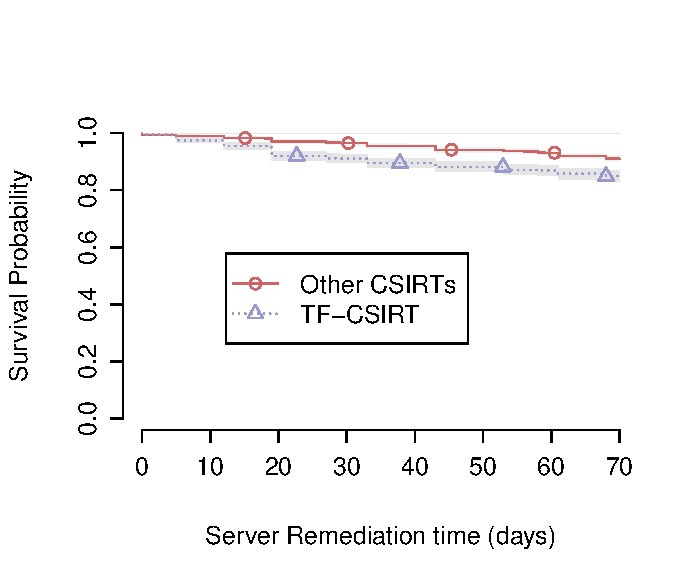
\includegraphics[width=.8\columnwidth]{tfcsirt_server.pdf}
\caption{Remediation rate of the DNS servers during the first campaign}
\end{figure}

\begin{figure}[!hbt]
\centering
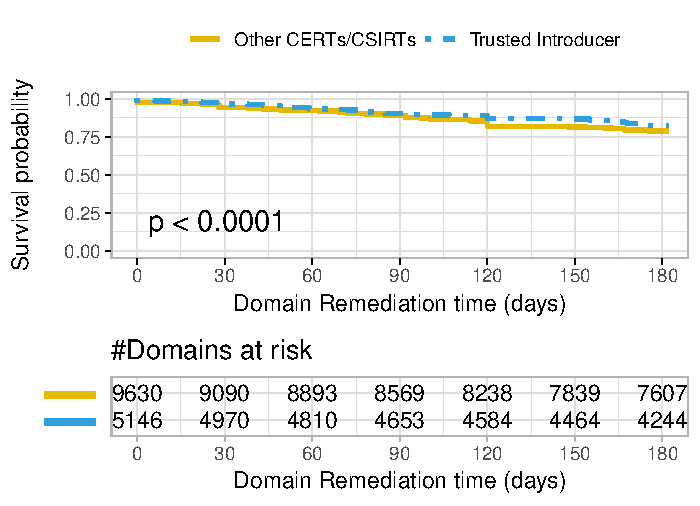
\includegraphics[width=.8\columnwidth]{tfcsirt_domain.pdf}
\caption{Remediation rate of the domains during the first campaign }
\end{figure}
\begin{figure}[!hbt]
\centering
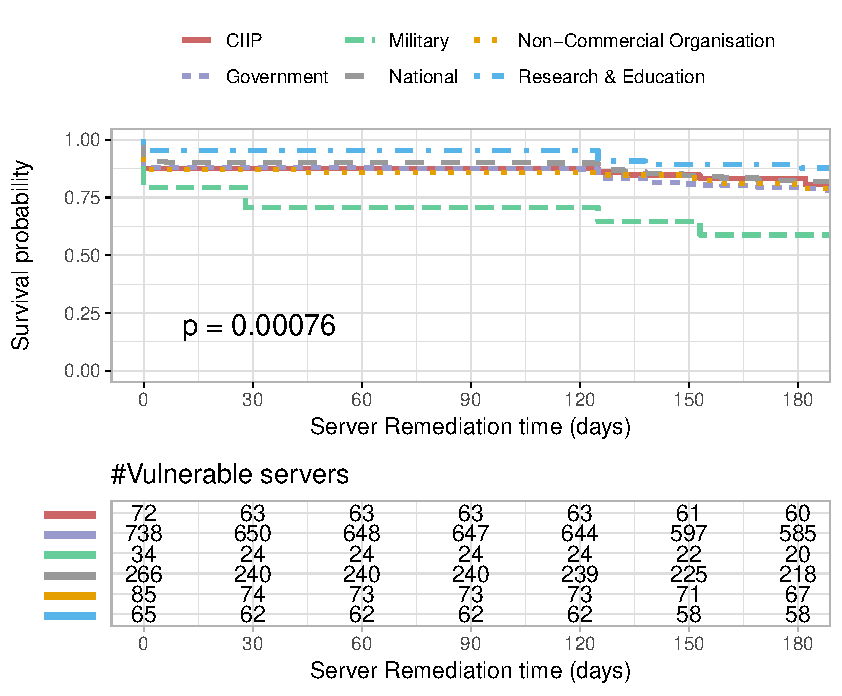
\includegraphics[width=.8\columnwidth]{figs/surv_tfcsirt-types.pdf}
\caption{Server remediation rate depending of the CSIRT constituency type }
\end{figure}


\subsection{Analyzing the remediation success}
\subsection{Lessons learned}